\begin{frame}[plain]
  \centering
  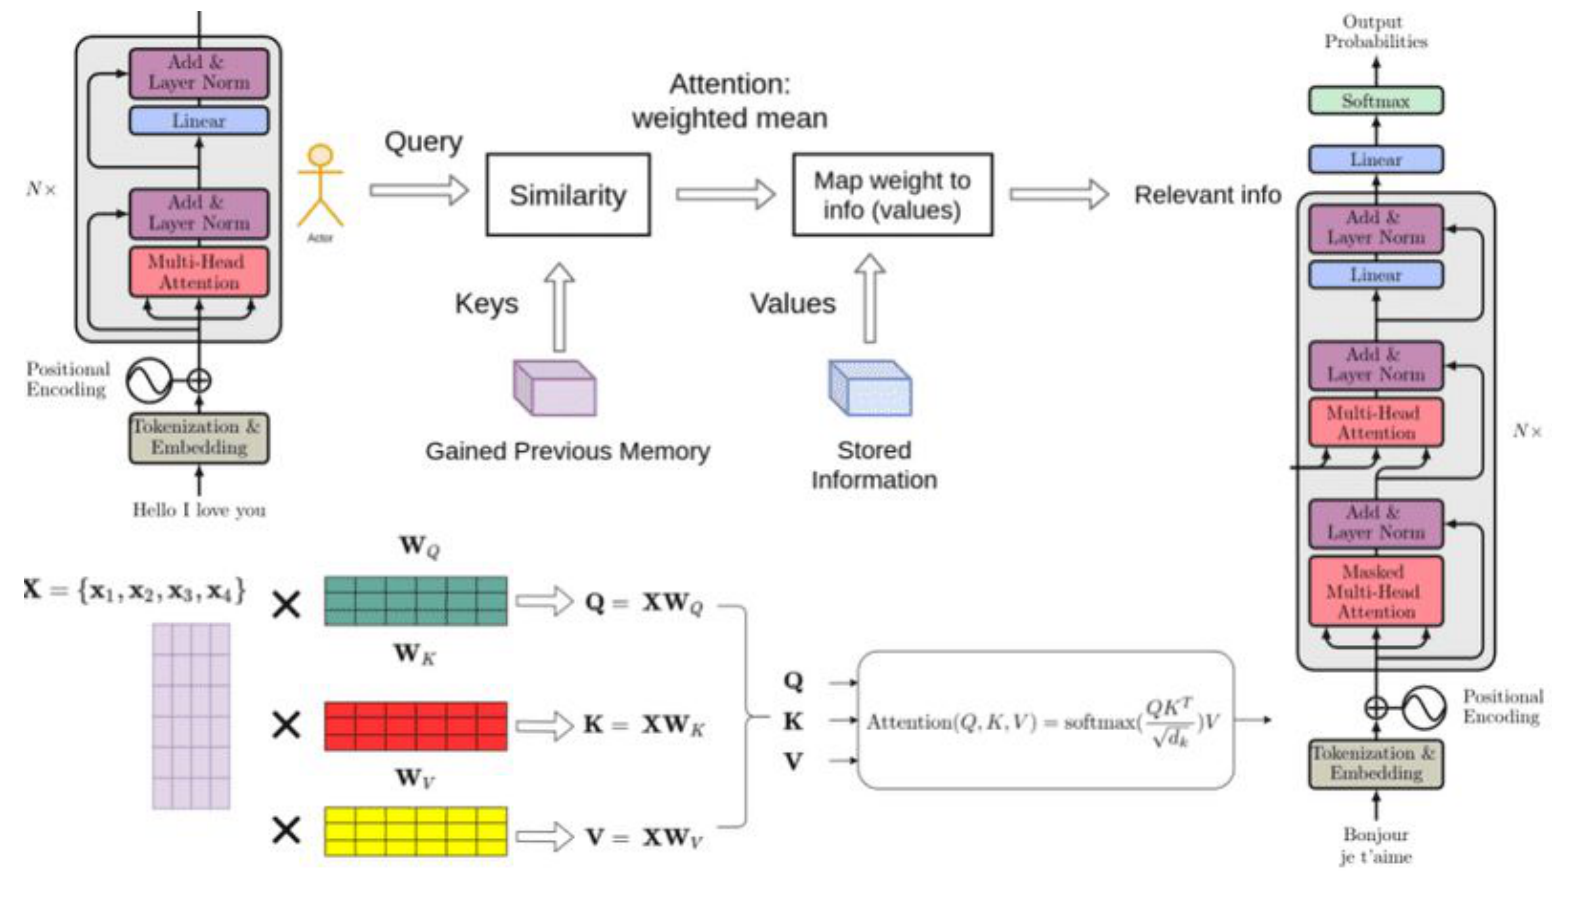
\includegraphics[width=\linewidth,height=0.95\paperheight,keepaspectratio]{images/introduction-to-transformers/transformer_attention_overview_qkv_architecture.png}
\end{frame}


\begin{frame}{Table of Contents}
  \small
  \begin{enumerate}[{\color{red}1.}]
    \setlength{\itemsep}{0.15em}
    \item {\color{red}Motivation}
    \item {\color{red}Learning Outcomes}
    \item {\color{red}Introduction to Transformers}
    \item {\color{red}Self-Attention Mechanism}
    \item {\color{red}Multi-Head Attention}
    \item {\color{red}Positional Encoding}
    \item {\color{red}Transformer Block}
    \item {\color{red}Encoder-Decoder Architecture}
    \item {\color{red}Causal Masking}
    \item {\color{red}Pre-LayerNorm vs.\ Post-LayerNorm Architectures}
    \item {\color{red}Layer Normalization vs RMSNorm}
    \item {\color{red}Transformer Variants}
    \item {\color{red}Limitations of Transformers}
    \item {\color{red}Summary}
  \end{enumerate}
\end{frame}
